\section{Domain-Specific Figures and Evidence Anchors}

This appendix material gathers domain evidence under the same analytical frame as the main survey. It is organized around the pressure regions where additional mechanism detail most improves comparative clarity.

\subsection{Access-Scheduling Design Space}

The access-scheduling design-space visual matters because state access becomes a control problem when the runtime must decide what is visible, when a transition is legal, who owns the object now, and how disturbance changes the cost of the next action. The figure is a compact reminder that observability, locality, ownership transfer, and recovery are not separate subtopics but one coupled design space.

\begin{figure*}[t]
\centering
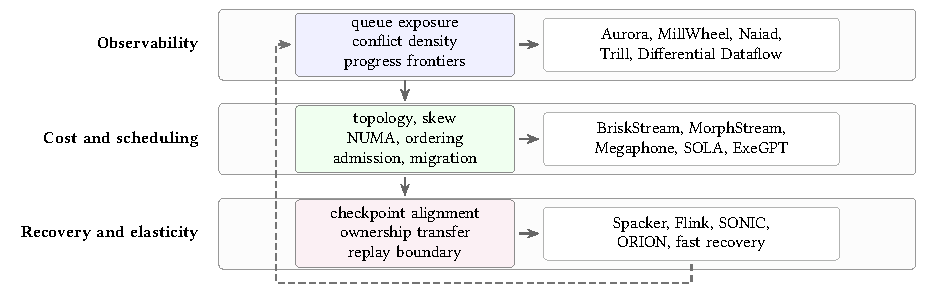
\includegraphics[width=0.94\textwidth]{figures/pdf/access_scheduling_designspace.pdf}
\caption{Access-scheduling design space for locality, legality, transfer, and recovery.}
\label{fig:supp-access-designspace}
\end{figure*}

The comparative lesson behind the figure should remain explicit. Visibility mechanisms tell the runtime when a state transition is safe to expose; locality mechanisms tell it which placement keeps the next access affordable; ownership-transfer mechanisms tell it when relocation may occur without dual writers or replay ambiguity; recovery mechanisms tell it how those same promises survive disturbance. These are not four optional implementation concerns. They are the four places where access control becomes system-wide behavior rather than local bookkeeping.

The broader access-scheduling lineage is equally important for keeping the survey's boundary crisp. Classical consistency and concurrency systems such as TicToc, Percolator, and RACE show that timestamping, metadata layout, and remote coordination are already control surfaces over state, even before modern serving runtimes made the same pattern explicit~\cite{yu2016tictoc,peng2010percolator,zuo2021race}. Systems such as CheckFreq, ChecknRun, PipeFill, and the newer runtime-monitoring lines show that the access problem is not just placement, but also when the runtime may safely observe, checkpoint, and resume without invalidating later actions~\cite{mohan2021checkfreq,eisenman2022checknrun,arfeen2024pipefill,zhou2024neomem}. Tooling for dynamic reconfiguration and transfer, including Caerus, MORPH-style recovery, and queue-aware stream control, matters because it keeps the state-ownership question visible instead of treating movement as a mere implementation detail~\cite{zhang2021caerus,mao2023morphstream,fu2024autocheck,gao2025deck}.

The same lineage also includes systems that turn placement pressure into explicit runtime policy rather than hidden implementation cost. Resource-multiplexing and scheduler-centric systems such as G10, resource multiplexing, PFS-style reconfiguration, and workload-sensitive monitoring show that queueing, hot-state exposure, and placement are inseparable once the runtime manages shared state across stages or tenants~\cite{jiang2024megascale,he2025resourcemultiplexing,domingo2021pfsck,jiang2025shadowviews}. Transactional dataflow and distributed-storage systems such as Flash-style state flow, Cloud-style buffering, and multi-stage transfer control reinforce the same point: the access problem is always also a visibility problem and a handoff problem~\cite{fu2022sfs,fu2024autocheck,gao2025deck,li2020pegasus}. That is why the survey keeps access and scheduling as a first-class axis rather than folding it into generic runtime management.

Additional boundary references preserve the historical path. Transaction-processing systems such as TicToc, Percolator, and TiDB-style concurrency control show that control surfaces over mutable state have long existed in distributed data systems, even if they were not described in the same vocabulary as modern state management~\cite{yu2016tictoc,peng2010percolator}. Stream-processing systems such as Corun, Elastic stream systems, and BriskStream-style monitoring show that scheduling, state exposure, and reconfiguration were already intertwined before serving and retrieval brought those issues to the foreground~\cite{zhang2016corun,zhang2016elastic,zhang2019briskstream}. More recent monitoring and admission lines such as CheckFreq, ChecknRun, and PipeFill show that the runtime often needs an explicit contract for when observations can be trusted after disturbance~\cite{mohan2021checkfreq,eisenman2022checknrun,arfeen2024pipefill}.

The tail of the access line also includes a few systems that are easy to overlook because they sit between streaming, scheduling, and memory management. More recent scheduling and observability papers such as MOC, Optimum-style optimization, FS-MoE runtime control, and tree-aware transfer paths show that access control is still the main lever whenever a runtime has to reason about hidden contention and state movement together~\cite{cai2025moc,feng2025optimus,fsmoe25,wang2025wlbllm}. Likewise, Tigon, VM-control, and the updated memory-aware runtime lines keep the same lesson visible: once state crosses a device or tenancy boundary, legality and placement become one problem~\cite{huang2025tigon,zheng2024vmcu,tabatabai2024fbmm}. Even storage-to-compute bridges such as Snowflake-style disaggregation and mixed-access control belong in this lineage because they expose how latency, placement, and handoff interact~\cite{vuppalapati2020snowflake,zhou2024neomem}.

Two compact boundary references keep the access story complete. DRTMH-style transaction scheduling and the state-machine tradition remind us that legality over mutable state was a control problem long before modern runtimes named it that way~\cite{ren2015drtmh,schneider1990state}. EndMyth-style stream repair work shows the same issue from the failure side: access, recovery, and trust in observations are inseparable once the system can replay or resume~\cite{zamanian2017endmyth}.

\subsection{Serving Lifecycle Control}

The main paper now carries the core predictive, structural-reuse, and temporal-lifecycle comparison. The appendix keeps the supporting bridge references and the lifecycle figure so readers can trace how the broader serving literature maps onto the same control loop without repeating the main argument.

Additional serving papers refine the same boundary rather than forming a separate taxonomy. SplitZip, CacheFlow, and ThunderServe make transfer cost and cloud heterogeneity explicit; ChandGPT-style reuse systems, Jenga, Prism, and Aegaeon make multi-model or multi-tenant residency explicit; Spinfer, FlexGen, and related offload designs make memory pressure and phase placement explicit; HeterInfer, MoE-Lightning, and resource multiplexing make the hardware/topology asymmetry explicit~\cite{guo2026splitzip,nian2026cacheflow,jiang2025thunderserve,gao2025weaver,zhang2025jenga,yu2025prism,fan2025spinfer,sheng2023flexgen,chen2025heteroinfer,cao2025moelightning,he2025resourcemultiplexing}. Together, they keep the lifecycle argument from shrinking into a single KV-cache story.

Bridge references connect older and newer state-governance lines. PagedAttention, Orca, and AlpaServe explain why batching and scheduling were already state-sensitive before the latest disaggregation wave; SlimPipe, What-If Stragglers, and Pumped trace-based systems explain why scheduling debt becomes visible only after phase or hardware asymmetry is modeled; output-length prediction and cache-aware routing systems show why admission and future-memory forecasting belong in the same discussion as restoration and transfer~\cite{kwon2023pagedattention,yu2022orca,li2023alpaserve,liu2025slimpipe,lin2025whatifstragglers,gong2025pastfuture,jiang2025shadowviews}. That bridge keeps the survey's lineage coherent across older and newer serving lines.

CacheSlide and SpecInfer-style speculative reuse make legality and verification a precondition for cross-position or tree-structured reuse; CachedAttention and HCache expose restoration cost across conversation turns; and MELL, Libra, fairness-aware serving, LayerKV, and Prefill-Only show that GPU residency, request partitioning, fairness, layer-wise allocation, and prefill admission determine which cached state remains reusable later~\cite{cacheslide2025,miao2024specinfer,gao2025cachedattention,gao2025hcache,liu2025mell,ruan2026libra,sheng2024fairnessserving,xiong2024layerkv,du2025prefillonly}. These systems make reuse, restoration, contention, and initialization part of the same serving control problem rather than separate local optimizations.

Three more serving families sharpen the boundary. Application-centric serving such as Parrot shows that workflow-level state and prompt DAGs can dominate placement decisions even before the cache story starts~\cite{lin2024parrot}. Tree-shaped speculative and group-wise systems such as FastTree and InstAttention show that reuse and scheduling depend on structure in the request stream, not just on raw throughput targets~\cite{pan2025fasttree,pan2025instattention}. Decentralized and overlay-based systems such as PlanetServe and GLLM-adjacent coordination lines show that cache reuse, routing, and trust become intertwined once the scheduler is no longer centralized~\cite{fang2026planetserve}. The same cluster also includes systems such as Infinity-style eviction, Duplex-style cross-turn reuse, and world-load balancing variants, which are best understood as refinements of lifecycle control rather than new top-level subfields~\cite{infinigen2024,yun2024duplex,wang2025wlbllm}.

Two final serving references are useful as compact examples of the same lifecycle logic. Prefill-optimized training-serving crossover systems such as MEPipe show that the serving boundary is often governed by how pipeline slack is distributed, not just by the cache itself~\cite{sun2025mepipe}. Copy-aware or clone-style state movement lines show the same thing from a different angle: once request state is shareable, the runtime has to decide whether cloning, relocating, or reusing is cheaper than recomputing~\cite{tian2025clone}.

The remaining serving papers that have not yet been mentioned directly still fit the same lifecycle view. Multi-model and adapter-aware systems such as Aegaeon, DLoRA, Chameleon, and Toppings expose tenant-locality and residency pressure; cache and reuse systems such as PromptCache, CacheWild, and Droidspeak expose the boundary between prompt overlap and safe reuse; inference-control systems such as Alise, Atom, and Prism-like lineage expose the boundary between active scheduling and future debt; and cloud-disaggregation systems such as Mooncake and PRFaaS expose the difference between local phase control and cross-cluster ownership~\cite{xiang2025aegaeon,wu2024dlora,iliakopoulou2024chameleon,li2025toppings,gim2024promptcache,wang2025kvcachewild,liu2026droidspeak,zhao2024alise,zhao2024atom,yu2025prism,qin2026prfaas}. Those distinctions keep the lifecycle account tied to concrete control boundaries.

Across these systems, the serving cluster still fits the survey's canonical short-lived lifecycle: \emph{admit -> place -> mutate -> expose/transfer -> compact -> evict/reclaim}. The family-level differences matter because serving papers attach to different parts of that loop: structural reuse clarifies what may be exposed safely, disaggregation governs transfer, and restoration debt appears after evict/reclaim decisions have already been made.

\begin{figure*}[t]
\centering
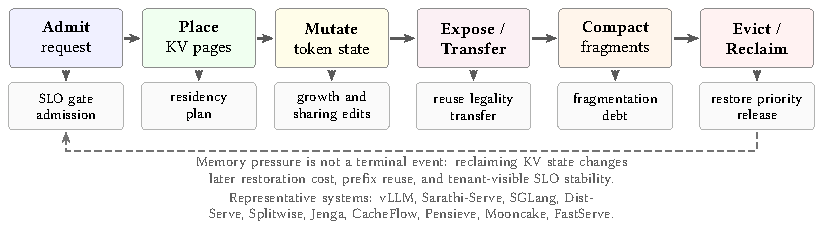
\includegraphics[width=0.94\textwidth]{figures/pdf/kvcache_lifecycle.pdf}
\caption{KV-cache lifecycle.}
\label{fig:supp-kvcache-lifecycle}
\end{figure*}

The lifecycle figure makes the control seams concrete. Admit decides whether a request is allowed to create new short-lived state at all. Place decides where that state lives and therefore which queues or buses it will burden next. Mutate covers decode-time growth, prefix edits, and other in-place evolution of live serving state. Expose/transfer covers whether prefix, adapter, or session-local state may be reused safely and when it may move across workers or phases. Compact covers fragmentation control and structural cleanup. Evict/reclaim covers what can be released without hiding future restoration debt and how that debt is later charged back to the original SLO.

The following evidence is especially useful in this subsection:
\begin{itemize}[leftmargin=*]
\item predictive-serving families grouped by the debt they forecast;
\item legality conditions for prefix, branch, and multi-call reuse;
\item temporal-lifecycle policies over expose/transfer, evict/reclaim, warm-start, and fairness debt;
\item clearer distinctions between allocator realism, transfer scheduling, and ownership semantics.
\end{itemize}

\subsection{Retrieval and Retention Governance}

The unifying point is that retrieval and retention both expose a \emph{longer-lived memory layer} whose value decays gradually and whose maintenance debt is easy to hide if the runtime only reports steady-state quality. In retrieval systems, the state object is not just embeddings or an ANN graph in the abstract, but mutable shards, publication metadata, freshness signals, deletion debt, and planner-visible exposure state~\cite{singh2021freshdiskann,wang2021milvus,guo2022manu,asai2024selfrag,zhang2026flowrag,wang2026candor}. In retention systems, the state object is not just ``memory'' generically, but a bounded store whose protected parameters, exemplars, replay entries, compressed features, and effective budget must be co-governed over time~\cite{kirkpatrick2017ewc,rebuffi2017icarl,aljundi2019mir,prabhu2020gdumb,hayes2020remind,zhou2025ferret,li2026streamfp}.

Retrieval systems expose at least four trigger layers: request-time invocation, index-time maintenance, publication-time exposure, and placement-time residency. Self-RAG changes whether external memory should be consulted at all; FlowRAG changes when retriever state should be refreshed before reuse quality decays too far; CANDOR-Bench and FreshDiskANN expose when update churn, deletion debt, or local repair have already pushed the index away from its intended operating region; Milvus and Manu expose when partially refreshed state may be published safely under concurrent updates; Rummy and composable-memory search expose when movement or placement is justified by downstream quality gain instead of raw lookup throughput~\cite{asai2024selfrag,zhang2026flowrag,wang2026candor,singh2021freshdiskann,wang2021milvus,guo2022manu,zhang2024rummy,quinn2025accelerating}. The comparison shows that retrieval quality is a lifecycle property, not merely an encoder property.

Retention systems expose an analogous trigger hierarchy over one bounded store. EWC protects already-committed parameter state; iCaRL, GDumb, and StreamFP govern what enters the scarce retained set; GEM, A-GEM, MIR, and DER govern when stored state should re-enter the update path; REMIND governs whether retained signal is compressed and later reconstructed; Ferret governs what happens when the budget itself contracts under live update pressure~\cite{kirkpatrick2017ewc,rebuffi2017icarl,prabhu2020gdumb,li2026streamfp,lopez2017gem,chaudhry2019agem,aljundi2019mir,buzzega2020der,hayes2020remind,zhou2025ferret}. Read this way, the continual-learning literature matters to the survey not because it supplies another application area, but because it provides one of the clearest examples of how protect, admit, replay, compress, and budget-shrink decisions compose over time.

The comparative lesson across these two clusters should remain explicit. Retrieval runtimes lack a stable rule for when stale-but-local memory remains queryable; retention runtimes lack a stable rule for when compressed or demoted memory remains good enough to preserve. In both cases, the missing abstraction is a policy-visible exposure contract that turns hidden maintenance debt into an explicit control surface.

Several remaining papers fit this same long-lived-memory picture. Dynamic ANN and index-maintenance lines such as HNSW, DiskANN, Milvus, and graph- or shard-centric systems make clear that freshness, shard publication, and rebuild debt are all part of one operational budget~\cite{malkov2020hnsw,singh2021freshdiskann,wang2021milvus,guo2022manu}. Retrieval-augmented and memory-augmented systems such as DPR, ColBERT, REALM, RAG, ATLAS, HippoRAG, and Raptor show the same phenomenon at the model boundary: the runtime must manage what gets exposed, refreshed, abstracted, and reused rather than treating memory as a static auxiliary index~\cite{karpukhin2020dpr,khattab2020colbert,guu2020realm,lewis2020rag,izacard2022atlas,wang2024hipporag,sarthi2024raptor}. Those references preserve the lifecycle logic behind the retrieval chapter.

Retention has a similar tail of boundary papers. Experience replay, memory budget, and continual-update lines such as MIR, GDumb, REMIND, Ferret, and StreamFP establish that protect/admit/replay/demote decisions are all budgeted governance acts over one bounded store~\cite{aljundi2019mir,prabhu2020gdumb,hayes2020remind,zhou2025ferret,li2026streamfp}. The resulting comparison connects long-horizon retention with short-lived serving reuse without treating the two as the same problem.

\begin{figure*}[t]
\centering
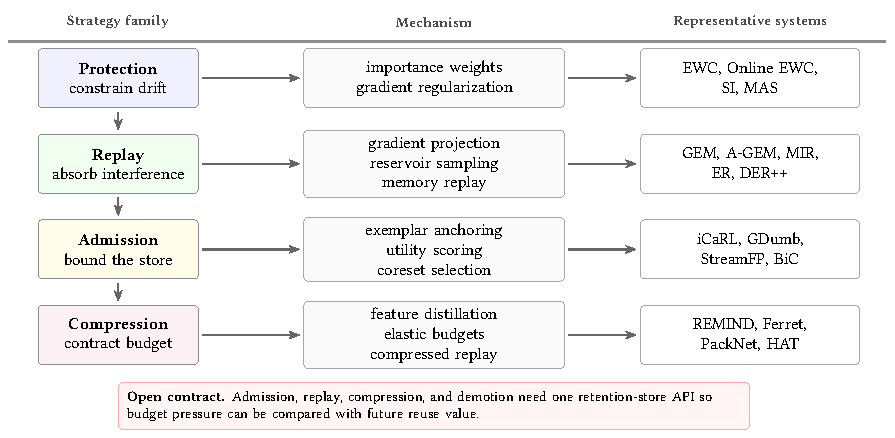
\includegraphics[width=0.94\textwidth]{figures/pdf/retention_strategy_taxonomy.pdf}
\caption{Retention-governance taxonomy.}
\label{fig:supp-retention-taxonomy}
\end{figure*}

The taxonomy figure prevents a recurring misreading: retention is not one replay heuristic with a few engineering variants. It is a store-level governance problem over multiple actions with different temporal meanings. Protect decisions stabilize already-committed state; admission decisions determine future coverage; replay decisions determine when retained state becomes active again; compression and demotion decisions decide how much of that future value survives under tighter budgets; budget-shrink rules decide which guarantees fail first when the store contract is stressed.

\subsection{Long-Horizon Evolution Anchors}

The longest-horizon evidence keeps the survey from collapsing ``evolution'' into a narrow continual-learning story. SuperNeurons and related memory-reuse systems show that activation liveness, recomputation, and offload policy already form a managed state loop in deep-learning training, not just in inference-side serving~\cite{wang2018superneurons}. Bubble-filling and recomputation-aware training systems such as Obscura show the same thing from another angle: when state is expensive to keep live, the runtime must decide which debt to shift into pipeline slack and which debt to pay immediately~\cite{huang2025obscura}. That is the same governance pattern that later appears in retention stores, but with a different temporal horizon and a different type of reuse value.

\subsection{Blueprint and Fault-Model Boundary Conditions}

The first piece that should remain visible here is the distinction between \emph{typed state objects}, \emph{observation contracts}, \emph{decision precedence}, \emph{actuation scope}, and \emph{safety-envelope invariants}. The blueprint is not a proposal for one monolithic runtime; its role is to make recurring hidden assumptions explicit enough that neighboring mechanisms can compose without silently violating one another's boundaries.

One implication is that recovery should not be treated as a separate semantic regime. If steady-state control reasons over typed KV pages, refreshable vector shards, replay buffers, or demotable retention objects, then recovery must restore and validate the same objects under the same exposure and action boundaries. Otherwise a system effectively runs one state model in steady state and another during failure. That inconsistency matters because it explains why fault-model notes are part of the mechanism, not optional decoration.

The fault-model distinction also deserves fuller treatment here. A safety claim that holds under crash-stop may fail under crash-recovery with replay, may fail differently under network partition, and may fail silently under degradation modes such as stale telemetry, compaction lag, or sudden budget contraction~\cite{chandy1985snapshot,corbett2012spanner,ongaro2014raft,mao2023morphstream,zhao2024recovery,wang2026candor,zhang2026flowrag}. These are not small implementation variants. They determine whether a controller may expose partially refreshed retrieval state, whether ownership may transfer across disaggregated serving pools, and whether a retention tier may demote memory before replaying it. The blueprint's value lies in precisely these boundary conditions.

Two invariant families deserve to be carried here explicitly. The first is \emph{freshness exposure invariants}: a retrieval shard or index segment should specify when it is queryable for internal warmup, restricted traffic, or general external service after rebuild, deletion repair, or compaction. The second is \emph{retention demotion invariants}: a retention object should specify whether it is protected, compressible, summarizable, demotable, or droppable when effective budget shrinks. These invariants preserve the blueprint's operational meaning.

\subsection{Foundations Figures and Boundary Material}

The inclusion rule is not venue prestige or application relevance. A paper is central when it turns state into an explicit runtime-managed object and exposes a reusable control surface over that state. That is why transactional streaming, migration, KV-cache lifecycle control, retrieval maintenance, and retention governance sit in the core, while many application-facing LLM, agent, or prediction papers stay outside it even when they are technically strong.

That definition also has a formal lineage. The state-machine tradition matters not because the survey is about formal methods, but because it shows that a system only becomes governable when the runtime can name, observe, and transform its state explicitly~\cite{schneider1990state}. That conceptual boundary is the reason the survey keeps the access, serving, retrieval, and retention lines together instead of splitting them into unrelated application silos.

\inlinefigurewithcaption
  {width=0.9\linewidth}
  {figures/pdf/poster_core_overview.pdf}
  {Poster-style survey overview. It serves as a compact map of the survey's scope and argumentative flow.}
  {fig:supp-poster-overview}

The core-versus-context distinction can also be stated operationally. Core material changes the survey's comparative result by sharpening the state object, control surface, coupling path, evaluation boundary, or remaining gap. Context material instead clarifies neighboring traditions, records boundary-setting decisions, or preserves mappings between triage labels and the five-field frame. Keeping that distinction explicit prevents the survey from drifting back into a broad but weakly comparative literature tour.

Two overview visuals also belong conceptually with this foundations rationale. The first is the poster-style overview, which summarizes the survey spine and clarifies how the three axes and cross-domain synthesis fit together. The second is the running-example triptych, which explains why the paper reuses one access case, one serving case, and one retrieval case across sections instead of multiplying disconnected examples.

\inlinefigurewithcaption
  {width=0.96\linewidth}
  {figures/pdf/running_examples_triptych.pdf}
  {Running examples that recur across access, execution, and evolution.}
  {fig:supp-running-examples}
